\documentclass[a4paper]{report}
%Uncomment this for better screen readable report 
%\documentclass[a4paper]{scrreprt}
\usepackage[english]{babel}
\usepackage[pdftex]{graphicx}
\title{Essig}
\author{
	Ewoud Kohl van Wijngaarden (s0113433)
	\and
	Wilfried van Asten (s0165883)
	\and
	Ruud Harmsen (s0165999)
	\and
	Mark Florisson (s0165972)
	\\
	\\
	\small Ontwerpproject (192199109) \\
	\small University of Twente \\
	\small Faculty of Electrical Engineering, Mathematics and Computer Science
}
\date{}

\begin{document}
\maketitle

\setcounter{tocdepth}{10}
\renewcommand\contentsname{Table of Contents}
\tableofcontents
\clearpage\selectlanguage{english}
\chapter{Introduction}
The ESSIG (Embedded Systems SImulator Generator) project is aimed
towards automating the process of writing a simulator for a
microcontroller. This means that the essig system will generate a
working simulator from a specification of a microcontroller given by
the user in an input language. Secondary targets include making the
simulator suitable for debugging programs and having the ability to
join several microcontrollers together in a network

\chapter{Related work}
Dit verslag beschrijft de bedachte programmeertaal Expr en beschrijft de
ontwikkeling van de bijbehorende compiler.

Aan het eind van het verslag zijn enkele appendices opgenomen.

\chapter{Overview}
Essig is roughly composed out of three components. First we have the
input language, which can be used to describe the micro controller a
simulator should be generated for. Than we have a generator, which
creates an implementation of the private API (see VM) that the VM can
use in simulating the micro controller. Than we have our VM, in which
the micro controller will be simulated. It exposes a public API to a
client which can then simulate programs like they were running on the
simulator. The following diagram illustrates how the components relate
to each other.

\begin{center}
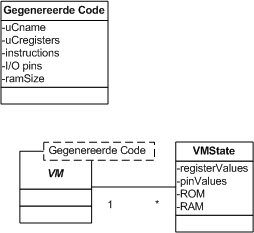
\includegraphics[width=5.376cm,height=4.932cm]{Essig-img002.png}
\end{center}
\chapter{AVR Microcontroller}
Dit verslag beschrijft de bedachte programmeertaal Expr en beschrijft de
ontwikkeling van de bijbehorende compiler.

Aan het eind van het verslag zijn enkele appendices opgenomen. 

\chapter{Grammar}
Dit verslag beschrijft de bedachte programmeertaal Expr en beschrijft de
ontwikkeling van de bijbehorende compiler.

Aan het eind van het verslag zijn enkele appendices opgenomen. 

\chapter{Simulator}
The final simulator is composed of two components: A general VM
containing things common to all microcontrollers and supplying debug
capabilities. All communication to the Simulator is done with a state
describing the current state of the simulator. The following
subsections describe each component in detail.

\section{VM}

The VM is a library in which functions are gathered that most simulators
have in common. These functions are defined in terms of a private API
for which implementations can be generated using the generator and the
definition language. Linked together they form a library that can run
programs like they were running on the simulated micro controller. It
is state driven in that most functions are parameterised with a state
which is then manipulated to the desired state by the function. This
design gives the client full freedom in manipulating and reading the
state, which when used properly gives interesting possibilities when
debugging a program.

\section{Micro Controller state}
To be able to let our VM execute any code for any microcontroller we
defined a structure that could represent any micro controller state. It
has all things that all micro controllers have in common. A RAM, a ROM,
some registers and pins. Our specification has all information needed
to generate this state and that is exactly what our VM does. Taking
compiled micro controller code it creates an initial state for the
micro controller specified in it generated component. This state is
then passed into every function that needs it to function (either
reading from it or manipulating it). This means that our VM can for
example manage and run several programs at the same time. We also have
a structure for diffs of this state. These diffs can be used to
backtrack the program execution. This relatively loose structure gives
a lot of interesting capabilities to the client (e.g. save a diffs
structure and state to the disk and resume exectution later on (with
full backtracking)).

\section{Generated code in the VM}
The generated portion of the VM works over a private API that the
generated code exports. This contains a lot of information (Like the
micro controller architecture information for the state), but more
importantly the opcode information. This is stored in small structures
that contains an instruction handler, a name and a mask. The
instruction handlers are private functions of the generated component,
but they all have the same signature as defined by the VM. The VM
passes execution on to this handlers when an instruction needs to be
executed (in the step or cont methods for example)and they then
manipulate the state through functions exported by the VM.

\section[Interrupt Handling]{Interrupt Handling}
Interrupts in essig can occur at two different levels:

\begin{enumerate}
\item {
From outside of the VM through the vm\_interrupt method }
\item {
From a peripharel }
\end{enumerate}
In either case a policy can govern whether or not the interrupt will be
passed on to the simulator

The simulator than enforces the actual rules for the microcontroller
that is simulated through a call to the handle\_interrupt method

After that the vm resumes normal execution
\section[Opcode parsing]{Opcode parsing}
In any simulator at some point opcodes will have to be parsed in order
to determine what code to execute. There are a lot of different
solutions to this problem and we will discuss a few of the here and
after that explain the solution we chose.

\subsection[Switch statement]{Switch statement}
To a lot of simulators out there this is the preferred method. The idea
is that you input the opcode or a part of the opcode into a switch
statement and continue execution at the matched case. This method has
one disadvantage: The case statement can't be generalized to any
simulator since the opcodes are (or can be) very different accross
different architectures.

\subsection{Some sort of function array}
This isn't used that much at all but for smaller architectures it can be
done. The idea is that you have an array of functions that handle an
opcode and that you index the array using the opcode. But as mentioned
for architectures with a relatively large opcode this array would
become far too large and since some instructions have some argument(s)
embedded in the opcode a lot of functions appear twice in the array.

\subsection{Our solution}
We wanted to be able to find our instruction in an array, but not have
an entry for every possible opcode. So we decided to make masks for
opcodes (these masks are then specified in the specification) and
before execution of the code match this to an instruction handler. This
process (lets call it disassembling) gives the advantage of fast opcode
resolution in exchange for a slightly longer load time. This idea is
further illustrated in the following diagram:

\section[PC incrementation]{PC incrementation}
In different micro controllers the program counter either points to the
current instruction or the next instruction. Because we delegate
program counter incrementation to our instruction handlers both
situations can be emulated quite easily by either incrementing the
program counter at the beginning of the instruction handler (to
indicate the next instruction) or at the end of the handler.

To illustrate this consider the following two pseudo code
implementations of rcall:

\begin{verbatim}
// PC points to next instruction}

PC = PC + 1

PUSH PC

PC = PC + k
\end{verbatim}

\begin{verbatim}
// PC points to current instruction}

PUSH (PC + 1)

PC = PC + k

PC = PC + 1
\end{verbatim}

It can be seen that in a micro controller in which the PC points to the
next instruction the push operation is simpler.

In the above example the effects of the instruction was exactly the same
but in micro controllers in which it is possible to push the PC (This
is not so in atmel micro controllers) there can be a difference:

\begin{verbatim}
// PC points to next instruction}

PC = PC + 1

STORE PC on stack
\end{verbatim}

\begin{verbatim}
// PC points to current instruction}

STORE PC on stack

PC = PC + 1
\end{verbatim}

Now in the first the top of the stack is the address of the next
instruction but in the second the address of the current instruction.
It also illustrates that our language can handle both situations
because the incrementation of the PC is handled by the instruction
handler

\chapter{User guide}
Dit verslag beschrijft de bedachte programmeertaal Expr en beschrijft de
ontwikkeling van de bijbehorende compiler.

Aan het eind van het verslag zijn enkele appendices opgenomen. 

\chapter{Limitations and future work}
Dit verslag beschrijft de bedachte programmeertaal Expr en beschrijft de
ontwikkeling van de bijbehorende compiler.

Aan het eind van het verslag zijn enkele appendices opgenomen. 

\bibliographystyle{plain}
\clearpage
\addcontentsline{toc}{chapter}{Bibliography}
\bibliography{Essig}

\appendix
\chapter[Grammar explanation]{Microcontroller specification language}
Op het laatste moment hebben we besloten om de ANTLR specificaties niet
uit te printen, test, test, test.

\chapter[Evaluation]{Evaluation}
De code en voorbeeldin- en uitvoer van een uitgebreid Expr programma is
\cite{atmelISA} opgenomen in deze appendix.
\end{document}

